\chapter{Effektivt val av aktörer för \\kravinsamling - Christoffer}

\section{Inledning}
I början av ett mjukvaruprojekt är det avgörande för projektets framgång att framställa en lista med krav som projektet ska uppnå. Detta är ett komplext ämne med mycket olika delar och metoder. Denna text diskuterar valet av stakeholders för kravinsamling och vilken prioritet dessa ges i processen.

\section{Syfte}
Syftet är att diskutera och jämföra den metod som vi använt i vårt projekt för framställning av krav med andra metoder. Detta för att kunna dra slutsattser om hur en mer sturkturerad metod för att välja stakeholders skulle påverkat vårt projekt och främst då kravframtagningsprocessen och dess resultat.

\section{Frågeställning}
Kan en sturkturerad medod för prioritering av krav och aktörer underlätta kravframtagning i ett mindre mjukvaruprojekt?

\section{Avgränsningar}
Denna jämförelse kommer att beröra den metod som använts i projektet för kravframställning och val av stakehoders med mer etablerade metoder. Det finns många oilka metoder så ett fåtal har valts ut för att visa på några olika vinklar. 

\section{Definitioner}
\begin{itemize}
	\item \textbf{Stakeholder} - Aktör med intresse av projektet.
	\item \textbf{LoFi-prototyp} - Snabb designprotoyp oftast tillverkad med penna och papper.
\end{itemize}


\section{Bakgrund}
Som analysansvarig i detta projekt har det varit mitt ansvar att kommunicera med både den egna projektgruppen och kunden för att framställa en kravspecifikation. Jag valde att lägga mest fokus på metoden för att ta fram olika krav mer än på vilka aktörer kraven skulle tas ifrån. Första aktörerna som vi kom i kontakt med var beställarna av projektet vilka gav oss en intiell kravlista. Senare i projektet fick vi möjlighet att intervjua tre potentiella slutanvändare. Denna intervju vände i stor utsträckning upp och ner på vår kravlista vilket fick mig att undersöka olika metoder för att välja och prioritera krav från olika stakeholders i ett projekt. Resultatet av denna undersökning presenteras i denna rapport.  

\section{Teori}
I denna del pressenteras en del teori som behövs för att senare kunna förstå och jämföra den metod vi använt i projektet med andra metoder och tekniker.

\subsection{Kravframställning}
Vid starten av ett mjukvaruprojekt börjar man analysera behoven för projektet för att formalisera en lista över krav som slutprodukten ska uppfylla. För att göra detta behövs det oftast att berörda aktörer, så kallade stakeholders, berättar vad de vill att produkten ska ha för funktioner och kvaliteter. En stakeholder kan vara vilken person som helst som blir påverkad av eller kan påverka utgången av projektet. Detta innebär att stakeholders kan vara  utvecklare, beställare, organisationsledare, olika experter och inte minst slutanvändare. 

Olika metoder som brainstorming, intervjuer och användartester, kan användas för att locka fram kraven från de olika aktörerna.

Olika stakeholders kan ha mycket olika krav på produkten. Detta skapar två olika problem, dels kan olika stakeholders ha luckor i kunskap om vilka krav som finns, och dels så kan olika aktörer ha olika åsikter om vilka krav som bör prioriteras. 

Lösningarna till detta är delvis motstridiga. För att inte missa några krav måste alla relevanta aktörer behandlas. Men ju fler aktörer som blir inblandade desto fler motstridiga krav riskerar att uppstå. Detta leder till att kraven måste analyseras och prioriteras beroende på vem som givit dem.
Till exempel kan det vara så att en utvecklare av programmet vill att akuta händelser markeras med lila för att det passar bäst in i programmets övriga färgschema. En av slutanvändrana tycker dock att det ska vara rött för det syns bättre. I detta fallet är det givetvis slutanvändarens krav som ska väga tyngre då det är denna person som kommer använda programmet. 
Om det gäller ett krav på vilket programspråk som ska användas däremot så lär utvecklarens, förmodligen större, kunskap inom ämnet göra att dennes åsikt väger tyngre.

\subsection{Urval av berörda aktörer}
För att effektivt framställa krav är det en viktigt att göra ett urval av aktörer som på bästa sätt kan skapa en komplett bild av projektets krav\cite{cs_choose_right}. Detta görs inte bara för att identifiera alla aktörer som är viktiga att ha med för att inte missa viktiga krav utan även för att se till att inte ta med aktörer vars åsikter och kunskap inte är nödvändiga för att skapa en komplett bild av projektet.

\subsection{Brainstorming}
Brainstorming är en metod för kravframtagning som görs i grupp. Syftet med brainstorming är att komma fram till en stor mängd idéer. Detta görs oftast tidigt i projektet eller när en helt ny del eller funktion ska utvecklas. I vårt projekt så har vi delat upp våra brainstormingtillfällen i två delar. Del ett är till för att storma idéer. Här är det öppet för alla idéer och inga idéer får skjutas ner eller kritiseras. Alla idéer skrivs upp i en lista oftast på en whiteboard. I del 2 så diskuteras de olika idéerna och filtreras ner till en eller några få idéer som sedan utvärderas vidare på olika sätt. Till exempel kan de gå vidare och bli prototyper eller så kan någon gruppmedlem efterforska vidare genom att läsa på om hur andra projekt har använt liknande idéer. 

\subsection{Intervjuer}\label{sec:ch-intervju}
Intervjuer kan läggas upp på flera olika sätt men ett av de vanligaste sätten är att förbereda ett antal frågor som behöver besvaras för att området för projektet ska kunna begränsas. Dessa frågor ställs sedan till de aktörer som har kunskap om det området. Frågorna kan antingen vara smala och direkta eller mer öppna. De smalare frågorna är bra för att få svar på specifika oklarheter. Till exempel ‘Behöver användare vara inloggade för att se schemat i programmet’. Den frågan kan bara besvaras med ‘ja’ eller ‘nej’ och skapar samtidigt ett tydligt krav som kan vidareutvecklas med följdfrågor. Mer öppna frågor är mer användbara när den som ställer frågorna behöver ett mer berättande svar.

\subsection{Användartest}
En metod som vi har använt en del är användartest utförda på Lo-Fi prototyper. Vad vi då typiskt gjort är att vi har presenterat ett antal olika prototyper för olika aktörer där de har kunnat navigera runt och testa olika designkoncept. Oftast har vi låtit användaren testa mer än en prototyp, där det har varit ett antal medvetna designskillnader, för att efter testet kunna få reda på vilket alternativ som användaren tyckte var bäst. Detta är utöver att hitta nya krav också ett bra sätt att validera de krav som redan samlats in.

\section{Metod}
\subsection{Vår framtagning}
Vår process för framtagning illustreras i en sorts tidslinje i figuren \ref{fig:ch_timeline}.

\begin{figure}[h]
	\centering
	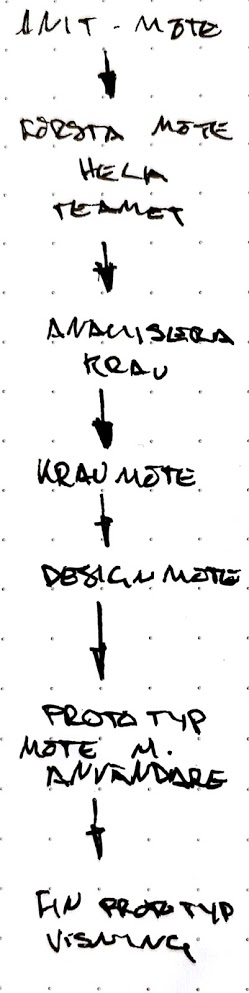
\includegraphics[height=0.7\textwidth]{Figures/timeline-christoffer.jpg}
	\caption{Tidslinje för kravframtagnin}
	\label{fig:ch_timeline}
\end{figure}

Vår process använde flera olika välbeprövade och väldokumenterade metoder för kravframtagning. Dessa användes under flera möten både internt i gruppen och med kund och användare. Däremot hade vi ingen tydlig process för att identifiera och kategorisera aktörer. Vi använde oss av en iterativ process för både krav och design där en intital idé presenterades och sedan förbättrades, tidsbrist gjorde dock att antalet iterationer blev ganska få. 

\section{Andra metoder}
De andra metoderna som jämförs i den här texten utgår alla ifrån att kategorisera de olika aktörerna i olika kategorier efter hur viktig deras inblandning är. I \cite{cs_novel} används tre kategorier lågt-, medel- och högt framträdande aktörer. \cite{cs_sturctured} anväder också tre kategorier men har istället obligatoriska, valbara och bra-att-ha aktörer.

\subsection{Metod 1}
I \cite{cs_novel} delas, som tidigare nämnt, aktörerna upp i tre kategorier. Denna metod beskriver främst hur krav kan prioriteras baserat på olika aktörers vikt i projektet.
Uppdeleningen sker baserat på hur många avgörande egenskaper aktörerna har. De avgörande egenskaperna är:
\begin{itemize}
	\item Aktören har makt över företaget
	\item Aktören blir direkt påverkad av projektet
	\item Aktören har viktiga krav på projektet
\end{itemize}

Om en aktör har en av dessa egenskaperna så hamnar den i den lägsta kategorin om den har alla tre så hamnar den i den högsta kategorin. Alla kattegorier viktas sedan och en formel används för att rangordna de olika aktörerna inom varje grupp. Baserat på detta så beräknas ett värde för varje aktör som används för att vikta deras krav och prioriteter. Processen utgår ifrån att krav redan finns och alla aktörer får betygsätta dessa i två steg, hur viktigt kravet är och hur snabbt det bör implemeteras. Betygen ges på en skala från 1 till 5. Denna siffra viktas med aktörens värde och alla värden slås sedan ihop för att skapa en prioritiserad lista med krav.

\subsection{Metod 2}
I \cite{cs_structured} beskrivs en strukturerad metod för att välja vilka aktörer som bör användas för kravframställning. 

Steg ett är att lista alla potentiella relevanta aktörer för hela projektet.
Därefter kategoriseras de in i de tre ovan nämnda kategorierna. Kategoriseringen sker genom att alla aktörer vars krav och erfarenhet är helt nödvändiga för ett lyckat projekt placeras i 'obligatoriska aktörer'. Alla aktörer som har bra kunskap i området eller på något sätt kan bidra med bra åsikter placeras i 'valbara aktörer'. Sist så placeras alla aktörer som inte har en viktig roll i utvecklandet och användandet av projektet i kategorin 'bra-att-ha aktörer. Dessa kan tillföra bra saker men är inte alls nödvändiga för projektets lyckande. 

Alla aktörer i kategorierna obligatoriska och valbara aktörer går vidare till nästa steg, de andra filtreras bort. Om det finns väldigt många aktörer kan ett mellansteg inkluderas där ett slumpmässigt urval görs.

Nu är det dags för första riktiga filtreringen, detta görs genom att aktörerna intervjuas. Syftet med intervjun är att bedöma aktörens kunskap och intresse. Dessa två viktas mot varandra för att välja ut de aktörerna som kan mest samtidigt som de är intresserade av projektet och villiga att bidra med sin kunskap och tid. Anledningen till att intresse undersöks så tidigt i processen är just att det kan ta väldigt mycket tid att jobba med kravframtagning och intresse är då av stor vikt för att orka delta under hela processen. 

I sista steget utvärderas de valda aktörernas kunskaper innom projektet, deras förmåga att kommunicera, deras förmåga att argumentera och deras sammarbetsförmåga. Denna utvärdering leder till en prioritiserad lista över aktörer.

\section{Resultat}
I denna del kommer vårt resultat från vår metod beskrivas.

\subsubsection{Inledande möte}
På det första mötet deltog vår teamledare, analysanvarige och kundens beställare, två personer anställda på avdelningen för test och innovation på Region Östergötland. Under detta möte avhandlades projektets övergripande syfte i breda drag.
Vi fick även reda på vilka olika kontaktpersoner vi skulle ha för olika frågor. De två deltagarna från kunden på detta mötet hade främst koll på tekniska detaljer och endast de övergripande detaljerna när det kom till mer funktionella krav.

\subsubsection{Första mötet med hela projektet}
På detta mötet var hela projektgruppen med samt, utöver de två beställarna från förra mötet, också en projektansvarig för ett större projekt i vilket vårt ingår som en mindre del. Denna projektansvarige, även jobbar inom kirurgi på sjukhuset, hade större kunskap om de funktionella kraven för projektet.

Utöver dessa deltagare fanns även två från kundens it-avdelning. Personerna från IT är dels de officiella beställarna men var även där för att kunna svara på frågor om tekniska och systemrelaterade frågor.

Vi använde intervjutekniken beskriven i avsnit\ref{sec:ch-intervju} med breda öppna frågor för att få en inledande idé om vad systemet skulle kunna. 

Efter detta möte så skrev projektledaren för det större projektet upp en lista med krav utifrån deras behov och det vi pratat om på mötet

\subsubsection{Analys av krav}
Kraven som guppen fick från kunden diskuterades sedan igenom i utvecklingsgruppen tillsammans med gruppens egna anteckningar från mötet. De analyserades och omformulerades därefter för att vara mer exakta och mätbara. Utöver det så kompletterades även kraven med gruppens egna mer tekniska krav som kunden inte hade tagit med.

\subsubsection{Kravmöte}
Efter analysen hade analysansvarig ännu ett möte med kunden där de nya och reviderade kraven gicks igenom och validerades.

\subsubsection{Designmöte}
Parallelt med kravframtagningen så jobbade gruppen på med olika protoyper för designen, detta går att läsa mer om i avsnitt \ref{sec:grafisk_design} i huvudelen samt i bilaga \ref{appendix:prototyp}.
Dessa protoyper presenterades och diskuderades på ett möte med kunden där analysansvarig deltog för att samla in ytterligare krav.

\subsubsection{Prototypdemo för användare}
Det var under detta möte som gruppen började inse att de initiala kraven hade ganska allvarliga brister. De krav som hade samlats in från produktägaren visade sig i flera avseenenden inte passa överens med det arbetsätt som användarna har. Trots detta så gjordes mycket få justeringar till kraven. Detta berodde dels på att det var relativt sent i projektet och utvecklingen behövde komma igång men det berodde också på att produktägarens åsikter värderades tyngre av gruppen.

\subsubsection{Demonstration av finprototyp}
Efter ett par veckor av utveckling demonstrerades en finprototyp för samma användare som vid förra mötet. Utöver användarna var även produktägaren och flera andra av kundens aktörer på plats. Finprototypen utgordes av en halvfärdig version av slutprodukten. Det fanns flera funktioner som var färdiga och som kunde visas upp i sin helhet. Ofärdiga funktioner visades helt enkelt inte upp.

Under detta möte insåg gruppen på allvar att de hade prioriterat fel krav för användarens behov.


\section{Diskussion}
Här kommer resutaten och mina åsikter att diskuteras och jämföras.

\subsection{De alternativa metoderna}
De alternativa metoderna som presenterats i denna text kompleterar varandra bra. Den som besbrivs i \ref{sec:cs_met1} är enbart avsedd för att prioritisera krav som finns. Det passar bra att kombinera med metoden i \ref{sec:sc_met2} då den har en bristfällig beskrivnin av hur krav bör prioriteras. Däremot har metod 2 en mycket tydlig process för att göra ett urval av aktörer, något som den första metoden saknar helt. 

\subsection{vår metod}
Att vi inte följde någon specifik process för att identifiera eller välja aktörer för kravframtagning berodde både på bristande erfarenhet men också tid. Trots detta fick vi ändå ihop bra krav som vi lyckades följa bra. Detta var dels för att gruppen var beredd att göra det bästa av de resurser vi fick tillgång till. Gruppen fick tillgång till betydligt mer aktörer än vad denna väntat sig och det ledde till att en mer strukturerad metod förmodligen hade uttnytjat potentialen bättre. Dock så hade den metod vi faktiskt använde också blivit bättre med tid för ytterligare en eller två itterationer.

\subsection{Implementera alternativa metoder}
Det går att se olika potentiella för-] och nackdelar med att använda de alternativa metoderna i denna text. En klar nackdel är att de skulle addera en hel del extra arbete. Men om tid hade funnits hade det definitivt hjälpt att lista alla aktörer i början och på ett mer metodiskt vis plockat fram krav från rätt aktörer.

Till viss del kan man också se att vi redan hade nytta av det som beskrivs. Till exempel så var alla aktörer som var med på kundmöten där frivilligt så alla aktörer vi hade att göra med låg högt på intreserad-skalan. 

Ett problem med att implementera prioritiseringen, både av krav och aktörer är att det hade varit svårt att applicera dessa tekninker på vissa situationer under projektet. Detta beror på att många aktörer som skulle fått samma prioritet i metod 1 skulle ha tyckt så olika att projektet skulle blivit aldeles för stort för den tid som fanns. Grunden till detta är att olika avdelningar på sjukhuset jobbar väldigt olika och avsikten med programmet var att det skulle passa alla avdeningar som jobbar med att planera operationer. 

Däremot hade förmodligen aldrig produktägarens åsikter prioriterats över slutanvändaren när det gällde gränssnit om vi hade haft en strukturerad metod för prioritisering.


\section{Slutsatser}
Som slutsats kan vi se att en sturkturerad metod för prioritisering av krav och aktörer vid kravframtagning kan underlätta processen. Det kan bidra med klarhet och det kan göra att felprioritering av krav undviks. Däremot kan det vara svårt att få plats med i utsatt tid om projektet är mindre. Det är heller inte lika i projekt med relativt få aktörer då det kan ta längre tid att filtrera aktörerna än att behandla alla. Således drar jag slutsattsen att det är viktigare ju större projektet är. I detta fallet var projektet i gränslandet och hade det varit aningen större så hade en strukturerad metod varit nödvändig. I detta fall så räckte det met nyfikna och intresserade aktörer som tillsammans skapade något bra. 




